\textbf{Qu'est ce qu'une variable ?} Les variables sont des symboles qui associent un nom à une valeur. La valeur est stockée dans la mémoire de l'ordinateur et le nom permet d'y accéder et/ou de modifier la valeur en tout temps. Une variable possède toujours un \textbf{type}. Ce dernier renseigne sur le "type" de la valeur stockée dans la variable. 

\begin{figure}[h!]
    \centering
    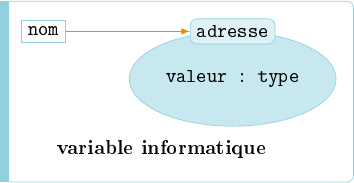
\includegraphics[width=7cm]{variable.png}
    \caption{Une variable}
    \label{variable}
\end{figure}

En \textsc{Python}, les noms de variables ne peuvent pas commencer par un chiffre, ni contenir d'espaces, ni contenir d'accents.

\begin{python}[caption = déclaration de variables]
nom_de_variable = valeur
#Exemples de variables correctes
variable1 = 1 #Une variable dont le nom est variable1 et la valeur est 1
b = "salut"
variable68452 = 0.50
variable_au_nom_tres_long = True
variable_lettre = 'a'
\end{python}


\subsection{Taille}

Les variables \textsc{Python} représentent une zone mémoire de l'ordinateur qui va stocker une certaine information. La taille d'une zone mémoire correspond à un ensemble de bits.

\begin{itemize}
    \item 1 \textit{bit} est le plus petit bout de donnée que l'on
    puisse stocker en mémoire. Il contient soit 1, soit 0.
    \item 1 octet (ou \textit{byte} en anglais) correspond à 8 bits
    \item 1 kilooctet (Ko) correspond à 1024 octets 
    \item 1 mégaoctet (Mo) correspond à 1024 Ko 
    \item 1 gigaoctet (Go) correspond à 1024 Mo 
\end{itemize}


\subsection{Type natif}\label{prim}

Python contient un ensemble de types natifs qui sont les types de données de \textbf{base}. Les types sont implicites lors de la déclaration d'une variable.

\begin{table}[!h]
    \centering
    \begin{tabular}{|c|c|}
        \hline
        Type & Description \\
        \hline
        \texttt{boolean} & Représente \textit{True} (vrai) ou \textit{False} (faux) \\
        \hline
        \texttt{str} & Représente une chaîne de caractères \\
        \hline
        %\texttt{byte} & & 1 octet \\
        %\texttt{short} & & 2 octets  \\
        \texttt{int} & Représente un entier\\
        %\texttt{long} & \multirow{-4}{*}{Représente un entier} & 8 octets \\
        \hline
        \texttt{float} & Représente un nombre à virgule\\
        %\texttt{double} & \multirow{-2}{*}{Représente un nombre à virgule} & 8 octets \\
        \hline
    \end{tabular}
    \caption{Type primitif}
    \label{table-primitifs}
\end{table}

\begin{python}[caption = Types de variables]
niveau = 'E'  #variable de type str
chaises = 12  #variable de type int
sonActif = False  #variable de type boolean
prixJeu = 12.50  #variable de type float
totalVoitures = 3453454  #variable de type int
\end{python}

Notons qu'on peut se renseigner sur le type d'une variable avec l'instruction \texttt{type(variable)}
\begin{python}[caption = Instruction type]
#Exemple
variable1 = 'a' 
variable2 = 2
variable3 = 12.50
print(type(variable1)) #Affiche "str"
print(type(variable2)) #Affiche "int"
print(type(variable3)) #Affiche "float"
\end{python}

\subsection{\textit{Cast} d'une variable}
Le mot \textit{cast} signifie qu'on impose un type à une variable. On impose un type à variable de la manière suivante :
\begin{python}[caption = Cast de variables]
nom_de_la_variable = type_que_je_veux(valeur)
#Exemples
a = int(1) # a est de type int
b = float(3) # b est de type float
c = float(4.5) # x est de type float
d = int(0.5) # Que se passe-t-il ?
\end{python}
%La raison qui pourrait nous pousser à faire ce choix est, par exemple, d'utiliser moins de mémoire pour représenter des variables qui en demandent moins. Si on s'en réfère au tableau \ref{prim}, on remarque qu'un \texttt{byte} consomme moins de mémoire qu'un \texttt{int} et que tous les deux permettent de représenter des entiers. On pourrait alors économiser de la mémoire en \textit{castant} nos variables en \texttt{byte} (\textsc{Python} représente les entiers par défaut en \texttt{int}).
Dans quels cas de figure est-ce utile de caster un nombre? Principalement parce qu'une opération s'effectue sur les mêmes types de données. On ne peut pas additionner "5" (la chaîne de caractères 5, un \texttt{str}!) avec 2 (un \texttt{int}!). Ici, on devrait donc d'abord caster le \texttt{str} en \texttt{int} avant l'opération. Mais il faut être prudent : que se passe-t-il si la chaîne de caractères ne peut être convertie en entier? Par exemple :
\begin{python}
int("salut") # Erreur!!!
\end{python}


\subsection{Affectation de variables}
Si vous avez bon souvenir, il était dit au tout début de la section \ref{variables} qu'on pouvait changer la valeur d'une variable. Pour ce faire, on égalise la variable à une nouvelle valeur. 
\begin{python}[caption = Réassignation de variables]
a = 2
print(a) #Affiche 2
a = 1
a = 4
print(a) #Affiche 4
a = "arbre" #Que se passe-t-il ?
print(a) #Affiche "arbre"
\end{python}

\subsection{Opérations arithmétiques}

On peut utiliser des opérateurs arithmétiques sur nos variables. Celles-ci vont être effectuées comme des opérations d'algèbre sur une calculatrice. Les opérations disponibles sont reprises dans le tableau ci-dessous
\begin{table}[!h]
    \centering
    \begin{tabular}{|c|c|}
        \hline
         Opération & Description\\
        \hline
        + & Addition \\
        \hline
        - & Soustraction \\
        \hline
        * & Multiplication \\
        \hline
        / & Division  \\
        \hline
        **  & Puissance \\
        \hline
        \% & Modulo \\
        \hline
    \end{tabular}
    \caption{Opérations arithmétiques}
    \label{oper}
\end{table}
\begin{python}
a = 4 + 6 #a vaut 10
a = ((a + a)/2)+1 #a vaut 11
b = a / 2 #b vaut 5
c = a**2 + b #c vaut 11^2 + 5 = 121 + 5 = 126
\end{python}


\subsection{Sucre syntaxique}

On dit souvent que les programmeurs sont des fainéants, et pour cause : ils cherchent à se faciliter la vie, et à réduire la taille des instructions qu'il tapent à longueur de journée! Ceux qui ont programmé les langages tel que \textsc{python} ont écrit des \textit{sucres syntaxiques} pour faciliter l'écriture et la lisibilité des programmes.

\begin{table}[!h]
    \centering
    \begin{tabular}{ccc}
        \texttt{x = x + 1} & $\Longleftrightarrow$ & \texttt{x += 1} \\
        \texttt{x = x + 1} & $\Longleftrightarrow$ & \texttt{x += 1} \\
        \texttt{x = x + 2} & $\Longleftrightarrow$ & \texttt{x += 2} \\
        \texttt{x = x - 2} &$\Longleftrightarrow$   & \texttt{x -= 2} \\
        \texttt{x = x / 2} &$\Longleftrightarrow$  & \texttt{x /= 2} \\
        \texttt{x = x * 2} &$\Longleftrightarrow$   & \texttt{x *= 2} \\

    \end{tabular}
    \caption{Quelques exemples de sucres syntaxiques}
\end{table}


\subsubsection{Exercices}

\begin{enumerate}
    \item successivement 
    \begin{enumerate}
    	\item $a = 124^3 + 27^2 + 7^3$
    	\item $b = 2589 \% 60$
    	\item $c =\frac{a^2 - b^3}{a}$
    	\item $a+b+c$
    \end{enumerate}

    \item Quelles est la valeur des différentes variables après l'exécution de
        cette partie de code?

\begin{python}
x = 10
y = x * 2
w = y - 10
z = y / w
\end{python}
\end{enumerate}